

\begin{enumerate}
	\item {Determine the following averages of the percentage of the population that are diagnosed with diabetes. Present your outputs clearly within your program with labels (explanatory text), not just the numbers by themselves. }
	\begin{enumerate}
		\item {Provincial averages (Ontario, Quebec, British Columbia, Alberta). One average per province (for all years and age groups).}
		\item {One national (Canada excluding territories) average for all years and age groups.}
		\item[\textbf{Output:}]
		\item[] {\begin{figure}[H]
			\includegraphics[width=12.75cm]{q1_ab.png}
		\end{figure}}
		\item[\textbf{Explaination:}]
		\item[] {{Once the program is executed, it opens the “statscan\_diabetes.csv” file and parses the data within the file. The program tokenizes each line in order the extract the year, the province, age group, gender and values for the group and stores them in an array of structs called “data\_set”, with each struct representing a single demographic group.} 
\\ \\
{Variables are then initialized for each province to calculate the averages in each province and the federal average using the data stored in the “value” struct. To calculate the averages, all of the values are summed up and divided by the total number entries (ignoring the lines with no data entered) and then the averages stored in the variables are printed.}}
		\item {Yearly averages (2015, 2016, 2017, 2018, 2019, 2020, 2021). One average per year (all age groups together) for each province and the whole country (Canada excluding territories) for a total of 35 averages.}
		\item[\textbf{Output:}]
		\item[] {\begin{figure}[H]
			\includegraphics[width=17cm]{q1_c.png}
		\end{figure}}
		\item[\textbf{Explaination:}]
		\item[] {To find the averages per year , variables were initialized to 0 for each year for each province. Then a nested loop is used to calculate and display the averages for each province per year.\\ \\ Within each loop, the code checks the year of the current data point and converts the string values using the atof function to double values.\\ \\The non-zero values are then summed up and divided by the number of values to calculate the year-wise averages. The averages are then displayed in a table.}
		\item {The average percentage of diabetes among age groups (35-49, 60-64, 65+). One average per age group (all years) for each province and the whole country (Canada excluding territories).}
		\item[\textbf{Output:}]
		\item[] {\begin{figure}[H]
			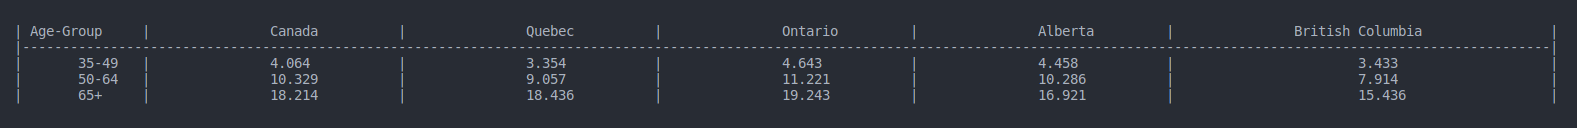
\includegraphics[width=17cm]{Q1_d.png}
		\end{figure}}
		\item[\textbf{Explaination:}]
		\item[] {The program defines several variables to hold the sums and averages for the different age groups (35 - 49, 50 - 64, and 65+) for the nation and the four provinces.\\ \\ Then, like the previous question uses nested for-loops to iterate over the data set and for each age group and province it sums up all of the non-zero values, calculates and displays the averages in a table.}
	\end{enumerate}
	\item {Determine which province has the highest percentage of diabetes (all years and age groups together as calculated in question 1a) and which province has the lowest percentage}
	\item[\textbf{Output:}]
	\item[] {\begin{figure}[H]
		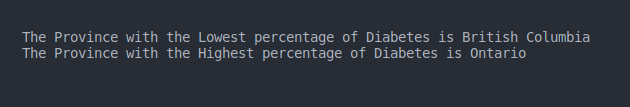
\includegraphics[width=12.75cm]{Q2.png}
		\end{figure}}
	\item[\textbf{Explaination:}]
	\item[] {The program defines variables to determine which province has the lowest and highest rates of diabetes. If and else if statements are used to compare all of the data from the variables. Then the variables are replaced with the highest and lowest averages respectively.}
	\item {Indicate the provinces that have diabetes percentages above the national average (Canada excluding territories) and the provinces that are below the national average.}
	\item[\textbf{Output:}]
	\item[] {\begin{figure}[H]
		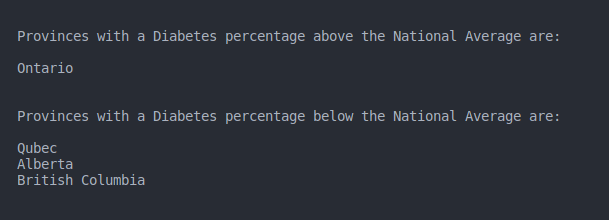
\includegraphics[width=12.75cm]{Q3.png}
		\end{figure}}
	\item[\textbf{Explaination:}]
	\item[] {The program recalls the national average and then uses if and else if statements to compare the earlier computed averages to the national average and displays which provinces are higher or lower than the national average.}
	\item {Indicate which year and province has the highest percentage of diabetes. Do the same for the lowest percentage. In case of a tie, you can mention multiple years and provinces.}
	\item[\textbf{Output:}]
	\item[] {\begin{figure}[H]
		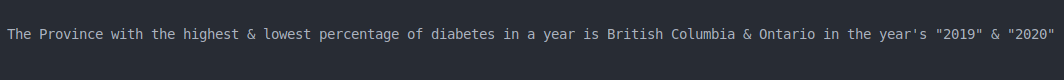
\includegraphics[width=15cm]{Q4.png}
		\end{figure}}
	\item[\textbf{Explaination:}]
	\item[] {Lowest and highest variables are initialized to zero and counter variables are defined.  The program loops through province averages and replaces the higher and lower values accordingly. It then prints out the provinces with the highest and lowest rates of diabetes and which years they occurred in.}	
\end{enumerate}



		
		
		